\documentclass[letterpaper]{article} % DO NOT CHANGE THIS
\usepackage{aaai24}  % DO NOT CHANGE THIS
\usepackage{times}  % DO NOT CHANGE THIS
\usepackage{helvet}  % DO NOT CHANGE THIS
\usepackage{courier}  % DO NOT CHANGE THIS
\usepackage[hyphens]{url}  % DO NOT CHANGE THIS
\usepackage{graphicx} % DO NOT CHANGE THIS
\urlstyle{rm} % DO NOT CHANGE THIS
\def\UrlFont{\rm}  % DO NOT CHANGE THIS
\usepackage{natbib}  % DO NOT CHANGE THIS AND DO NOT ADD ANY OPTIONS TO IT
\usepackage{caption} % DO NOT CHANGE THIS AND DO NOT ADD ANY OPTIONS TO IT
\frenchspacing  % DO NOT CHANGE THIS
\setlength{\pdfpagewidth}{8.5in}  % DO NOT CHANGE THIS
\setlength{\pdfpageheight}{11in}  % DO NOT CHANGE THIS
\usepackage{algorithm}
\usepackage{algpseudocode}

\usepackage{newfloat}
\usepackage{listings}
\DeclareCaptionStyle{ruled}{labelfont=normalfont,labelsep=colon,strut=off} % DO NOT CHANGE THIS
\lstset{%
	basicstyle={\footnotesize\ttfamily},% footnotesize acceptable for monospace
	numbers=left,numberstyle=\footnotesize,xleftmargin=2em,% show line numbers, remove this entire line if you don't want the numbers.
	aboveskip=0pt,belowskip=0pt,%
	showstringspaces=false,tabsize=2,breaklines=true}
\floatstyle{ruled}
\newfloat{listing}{tb}{lst}{}
\floatname{listing}{Listing}


\setcounter{secnumdepth}{0} %May be changed to 1 or 2 if section numbers are desired.



\title{



Physics-informed Representation and Learning: Control and Risk Quantification
}
\author{
    Zhuoyuan Wang\textsuperscript{\rm 1},
    Reece Keller\textsuperscript{\rm 1},
    Xiyu Deng\textsuperscript{\rm 1}, Kenta Hoshino\textsuperscript{\rm 2}, Takashi Tanaka\textsuperscript{\rm 3}, Yorie Nakahira\textsuperscript{\rm 1}
}
\affiliations{
    \textsuperscript{\rm 1}Carnegie Mellon University,
    \textsuperscript{\rm 2}Kyoto University,
    \textsuperscript{\rm 3}University of Texas at Austin
    \\


    \{zhuoyuaw, rdkeller, xiyud\}@andrew.cmu.edu, hoshino@i.kyoto-u.ac.jp, ttanaka@utexas.edu, yorie@cmu.edu
}

\iffalse
\title{My Publication Title --- Single Author}
\author {
    Author Name
}
\affiliations{
    Affiliation\\
    Affiliation Line 2\\
    name@example.com
}
\fi

\iffalse
\title{My Publication Title --- Multiple Authors}
\author {
    First Author Name\textsuperscript{\rm 1},
    Second Author Name\textsuperscript{\rm 2},
    Third Author Name\textsuperscript{\rm 1}
}
\affiliations {
    \textsuperscript{\rm 1}Affiliation 1\\
    \textsuperscript{\rm 2}Affiliation 2\\
    firstAuthor@affiliation1.com, secondAuthor@affilation2.com, thirdAuthor@affiliation1.com
}
\fi




\usepackage{xcolor}
\usepackage{amsmath}
\usepackage{amsthm}
\usepackage{amsfonts}
\usepackage{graphicx}
\usepackage{caption}
\usepackage{subcaption}
\usepackage{bm}

\newcommand{\todo}[1]{\textcolor{blue}{[TODO: #1]}}
\newcommand{\jacob}[1]{\textcolor{blue}{[Jacob: #1]}}
\newcommand{\overview}[1]{{\leavevmode\color{red}#1}}
\newcommand{\resolved}[1]{}

\newcommand{\ie}{\textit{i.e., }}
\newcommand{\eg}{\textit{e.g., }}
\newcommand{\pr}{\mathbb{P}}
\newcommand{\safe}{\mathcal{C}}

\DeclareMathOperator*{\argmax}{arg\,max}
\DeclareMathOperator*{\argmin}{arg\,min}


\newtheorem{theorem}{Theorem}
\newtheorem{lemma}[theorem]{Lemma}
\newtheorem{proposition}[theorem]{Proposition}
\newtheorem{corollary}[theorem]{Corollary}
\newtheorem{definition}[theorem]{Definition}
\newtheorem{remark}[theorem]{Remark}
\newtheorem{assumption}[theorem]{Assumption}

\usepackage{tikz}
\usepackage{xcolor}
\usepackage{verbatim}
\usepackage{multirow}
\usepackage{color}
\usepackage{colortbl}
\usepackage{pgfplots}
\DeclareUnicodeCharacter{2212}{}
\usepgfplotslibrary{groupplots,dateplot}
\usetikzlibrary{patterns,shapes.arrows}
\pgfplotsset{compat=newest}
\usetikzlibrary{shapes.arrows}
\usetikzlibrary{arrows.meta}
\usetikzlibrary{positioning, fit, shapes.geometric}
\usetikzlibrary{backgrounds}
\definecolor{newblue}{RGB}{189,215,239}
\definecolor{newgray}{RGB}{214,214,214}
\definecolor{neworange}{RGB}{241,205,177}
\definecolor{newyellow}{RGB}{251,231,163}
\definecolor{newgreen}{RGB}{202,223,184}
\definecolor{cmured}{RGB}{196,18,48} % Red
\definecolor{cmuskibored}{RGB}{147,17,32} % Skibo Red
\definecolor{cmuyellow}{RGB}{253,181,21} % Yellow
\definecolor{cmublue}{RGB}{4,54,115} % Blue
\definecolor{cmutan}{RGB}{188,180,158} % Tan
\definecolor{cmuteal}{RGB}{31,76,76} % Teal
\definecolor{cmugreen}{RGB}{113,159,148} % Green
\definecolor{cmuskyblue}{RGB}{0,123,192} % Sky Blue
\definecolor{cmuirongray}{RGB}{109,110,113} % Iron Grey
\definecolor{cmugray}{RGB}{244,244,244} % Iron Grey
\usepackage{pgfplots}
\usepackage{makecell}
\usepgfplotslibrary{fillbetween}
\begin{filecontents*}{pinn_epoch.dat}
    x y err
    10000  7.104  0.025882
    20000  5.322  0.02009
    30000  5.475  0.02065
    40000  5.940  0.022517
    50000  4.733  0.018146
    60000  4.809 0.018371
\end{filecontents*}
\begin{filecontents*}{pinn_pde.dat}
    x y err
    100 5.498 0.020817
    200 5.391 0.02022523
    300 5.749 0.02171
    400 5.927 0.022209
    500 5.478 0.02058
    600 5.283 0.019888
    1200 5.153 0.01962
    2400 4.992 0.01894
\end{filecontents*}
\begin{document}

\maketitle

\begin{abstract}
Optimal and safety-critical control are fundamental problems for stochastic systems, and are widely considered in real-world scenarios such as robotic manipulation and autonomous driving. In this paper, we consider the problem of efficiently finding optimal and safe control for high-dimensional systems. Specifically, we propose to use dimensionality reduction techniques from a comparison theorem for stochastic differential equations together with a generalizable physics-informed neural network to estimate the optimal value function and the safety probability of the system. The proposed framework results in substantial sample efficiency improvement compared to existing methods. We further develop an autoencoder-like neural network to automatically identify the low-dimensional features in the system to enhance the ease of design for system integration. We also provide theoretical analysis and experiments to validate the efficacy of the proposed method.

\end{abstract}

\section{Introduction}

Optimal control and safety-critical control are the two central concerns for autonomous systems.
These concerns are particularly pronounced in real-world applications, including manufacturing robots and autonomous cars.
The operational environment often introduces stochastic noise, which compounds the difficulties of achieving optimal performance and ensuring safety. Traditional deterministic methods prove inadequate for stochastic dynamics~\cite{katsoulakis2020data}.
Furthermore, many real-world systems are characterized by high-dimensional state spaces (\eg multi-agent systems), leading to substantial computational burdens when devising optimal and safe control strategies.


Previous work on stochastic optimal control deals with diverse uncertainty and randomness, but these methods are not efficient for high-dimensional systems because forward rollouts and backward dynamic programming requires computation that scales exponentially with the dimension of the state.~\cite{gorodetsky2018high, frankowska2020necessary}\resolved{to elaborate}.
Previous studies on stochastic safe control aim to control the level of risk in the system for a certain period of time, and ensure the probability of safety does not decay over time~\cite{samuelson2018safety,gomez2016real}.
These methods rely on accurate estimation of the probability of risk in the system, and standard methods for such risk estimation are computationally heavy, especially for high-dimensional systems.
For both problems, existing methods require computation that scales linearly with the time horizon of interest. To the best of our knowledge, there is no study that provides generalization of the value function and risk probability in the time horizon, which can be very beneficial for efficient computation in systems with long-term performance requirements.

In order to address these challenges, this study proposes a unified framework to efficiently estimate the value function and safety probability of high-dimensional stochastic systems. The method leverages a comparison theorem~\cite{10.1215/kjm/1250523321} to find low-dimensional representations of the value function and safety probability, and uses such low-dimensional features to construct low-dimensional partial differential equations (PDEs) for the value function and safety probability calculation in order to reduce the dimension of the problem for efficient computation.
We further propose a physics-informed neural network (PINN) to solve these PDEs for better sample complexity and generalization abilities.
We also propose an autoencoder-like neural network to automatically identify low-dimensional features of the system, and provide error analysis incurred from the process.
Fig.~\ref{fig:overall_diagram} shows the overall diagram of the proposed method.
The advantages of the proposed method are
\begin{enumerate}
    \item A unified framework for accurate estimation of value functions and safety probabilities of stochastic systems (Fig.~\ref{fig:PINN diagram}).
    \item Efficient estimation with much lower sample complexity for high-dimensional systems (Fig.~\ref{fig:sample_complexity}).
    \item Generalization to unseen regions in the state space and longer time horizons (Fig.~\ref{fig:value_func_visual} and Fig.~\ref{fig:safe_prob_3d->2d}).
    \item Intuitive plug and use with automatic feature identification (Fig.~\ref{fig:AE diagram}).
\end{enumerate}

\begin{figure}
    \centering
    %%%%%%%%%%
% by Xiyu
%%%%%%%%%%%

% color
\definecolor{color5}{HTML}{F2CC8F}
\definecolor{color2}{HTML}{F4F1DE}
\definecolor{color3}{HTML}{3D405B}
\definecolor{color4}{HTML}{81B29A}
\definecolor{color1}{HTML}{E07A5F}
\tikzset{
diagonal fill/.style 2 args={fill=#2, path picture={
\fill[#1, sharp corners] (path picture bounding box.south west) -|
                         (path picture bounding box.north east) -- cycle;}},
reversed diagonal fill/.style 2 args={fill=#2, path picture={
\fill[#1, sharp corners] (path picture bounding box.north west) |- 
                         (path picture bounding box.south east) -- cycle;}}
}

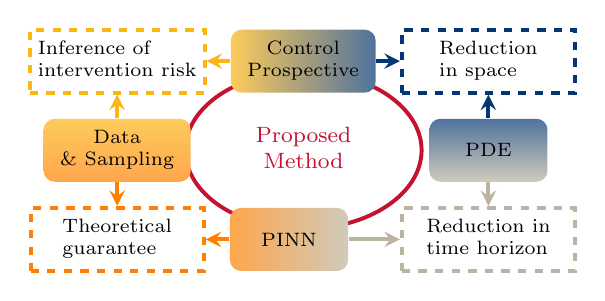
\begin{tikzpicture}[
    node distance = 4cm,
    node/.style={circle, fill=#1, inner sep=2pt, minimum size=0.7cm}, 
    edge/.style={-stealth, #1}
]

% 
\node[rectangle, draw=cmuyellow, dashed, line width=0.5mm, minimum height=0.8cm,minimum width=2.2cm,inner sep=-3pt] (t1){\scriptsize \begin{tabular}{ll}
% Observed data \\ to infer vs \\ the risk of\\ intervention.
Inference of \\ intervention risk
\end{tabular}};
\node[shading = axis, rectangle, left color= cmuyellow!70, right color= cmublue!70, minimum height=0.8cm,minimum width=1.5cm, rounded corners,inner sep=0pt] (control)[right=0.3cm of t1] {\scriptsize \begin{tabular}{cc}
Control \\ Prospective
\end{tabular}};

\node[rectangle, draw=cmublue, dashed, line width=0.5mm, minimum height=0.8cm,minimum width=2.2cm,inner sep=0pt] (t2) [right=0.3cm of control]{\scriptsize \begin{tabular}{ll}
Reduction \\ in space
\end{tabular}};

\node[shading = axis, rectangle, top color= cmuyellow!70, bottom color= orange!70, minimum height=0.8cm,minimum width=1.5cm, rounded corners, inner sep = 0pt] (sr) [below=0.3cm of t1] {\scriptsize \begin{tabular}{cc}
Data \\ \& Sampling\\
\end{tabular}};

\begin{scope}[on background layer]
\node[ellipse, draw = cmured, line width=0.5mm, minimum width = 3cm, minimum height = 2cm, rounded corners] (pm)[right= -0.1 cm of sr]{\footnotesize \textcolor{cmured}{\begin{tabular}{cc}
Proposed \\Method
\end{tabular}}};
\end{scope}

\node[shading = axis, rectangle, top color= cmublue!70, bottom color= cmutan!70, minimum height=0.8cm,minimum width=1.5cm, rounded corners] (pde) [below=0.3cm of t2] {\scriptsize PDE};

\node[rectangle, draw=orange, dashed, line width=0.5mm, minimum height=0.8cm,minimum width=2.2cm,inner sep=0pt] (t3)[below=0.3cm of sr]{\scriptsize \begin{tabular}{ll}
Theoretical \\ guarantee
\end{tabular}};

\node[shading = axis, rectangle, left color= orange!70, right color= cmutan!70,  minimum height=0.8cm,minimum width=1.5cm, rounded corners] (pinn)[right=0.3cm of t3]{\scriptsize PINN};

\node[rectangle, draw=cmutan, dashed, line width=0.5mm, minimum height=0.8cm,minimum width=2.2cm] (pw)[below=0.3cm of pde,inner sep=0pt]{\scriptsize \begin{tabular}{ll}
% Reduction in \\ time horizon \\due to PDE\\ constrains.
Reduction in \\ time horizon 
\end{tabular}};

%Edges
\draw[edge=cmuyellow,line width=0.5mm] (control) -> (t1);
\draw[edge=cmublue,line width=0.5mm] (control) -> (t2);
\draw[edge=cmuyellow,line width=0.5mm] (sr) -> (t1);
\draw[edge=cmublue,line width=0.5mm] (pde) -> (t2);
\draw[edge=orange,line width=0.5mm] (pinn) -> (t3);
\draw[edge=cmutan,line width=0.5mm] (pde) -> (pw);
\draw[edge=cmutan,line width=0.5mm] (pinn) -> (pw);
\draw[edge=orange,line width=0.5mm] (sr) -> (t3);
\end{tikzpicture}


% \begin{tikzpicture}[
%     node distance = 4cm,
%     node/.style={circle, fill=#1, inner sep=2pt, minimum size=0.7cm}, 
%     edge/.style={-stealth, #1}
% ]

% % 
% \node[rectangle, fill=newyellow,  line width=0.5mm, minimum height=0.8cm,minimum width=1.8cm,inner sep=-3pt] (t1){\scriptsize \begin{tabular}{ll}
% % Observed data \\ to infer vs \\ the risk of\\ intervention.
% Inference of \\ cost and risk
% \end{tabular}};

% \node[rectangle,  draw, line width = 0.3mm, minimum height=0.8cm,minimum width=1.8cm, inner sep=0pt] (control)[right=0.5cm of t1] {\scriptsize \begin{tabular}{cc}
% Control \\ Prospective
% \end{tabular}};

% % \node[rectangle,draw=cmuyellow,dash pattern= on 3pt off 5pt,line width = 0.3mm, minimum height=0.8cm,minimum width=1.8cm, inner sep=0pt,postaction={draw,cmublue,dash pattern= on 3pt off 5pt,dash phase=4pt,thick}] (control)[right=0.3cm of t1] {\scriptsize \begin{tabular}{cc}
% % Control \\ Prospective
% % \end{tabular}};


% \node[rectangle, fill=newblue,  line width=0.5mm, minimum height=0.8cm,minimum width=1.8cm,inner sep=0pt] (t2) [right=0.5cm of control]{\scriptsize \begin{tabular}{ll}
% Reduction \\ in space
% \end{tabular}};

% \node[draw, line width = 0.3mm, rectangle, minimum height=0.8cm,minimum width=1.8cm,  inner sep = 0pt] (sr) [below=0.3cm of t1] {\scriptsize \begin{tabular}{cc}
% Data \\ \& Sampling\\
% \end{tabular}};

% % \node[rectangle,draw=orange,dash pattern= on 3pt off 5pt,line width = 0.3mm, minimum height=0.8cm,minimum width=1.8cm, inner sep=0pt,postaction={draw,cmuyellow,dash pattern= on 3pt off 5pt,dash phase=4pt,thick}] (sr)[below=0.3cm of t1] {\scriptsize \begin{tabular}{cc}
% % Data \\ \& Sampling\\
% % \end{tabular}};

% % \begin{scope}[on background layer]
% % \node[rectangle, line width=0.5mm, minimum width = 3cm, minimum height = 2cm, rounded corners] (pm)[right= -0.1 cm of sr]{\scriptsize \begin{tabular}{cc}
% % Proposed \\Method
% % \end{tabular}};
% % \end{scope}

% \node[rectangle, minimum height=0.8cm,minimum width=1.8cm,  inner sep = 0pt] (pm) [below=0.3cm of control] {\footnotesize \begin{tabular}{cc}
% \underline{Proposed Method}
% % Proposed Method
% \end{tabular}};

% \node[rectangle, draw, line width = 0.3mm, minimum height=0.8cm,minimum width=1.8cm] (pde) [below=0.3cm of t2] {\scriptsize PDE};

% % \node[rectangle,draw=cmublue,dash pattern= on 3pt off 5pt,line width = 0.3mm, minimum height=0.8cm,minimum width=1.8cm, inner sep=0pt,postaction={draw,cmutan,dash pattern= on 3pt off 5pt,dash phase=4pt,thick}] (pde)[below=0.3cm of t2] {\scriptsize \begin{tabular}{cc}
% % PDE
% % \end{tabular}};

% \node[rectangle, fill=neworange,  line width=0.5mm, minimum height=0.8cm,minimum width=1.8cm,inner sep=0pt] (t3)[below=0.3cm of sr]{\scriptsize \begin{tabular}{ll}
% Theoretical \\ guarantee
% \end{tabular}};

% \node[rectangle, draw, line width = 0.3mm,  minimum height=0.8cm,minimum width=1.8cm] (pinn)[right=0.5cm of t3]{\scriptsize PINN};

% % \node[rectangle,draw=cmutan,dash pattern= on 3pt off 5pt,line width = 0.3mm, minimum height=0.8cm,minimum width=1.8cm, inner sep=0pt,postaction={draw,orange,dash pattern= on 3pt off 5pt,dash phase=4pt,thick}] (pinn)[right=0.3cm of t3] {\scriptsize \begin{tabular}{cc}
% % PINN
% % \end{tabular}};

% \node[rectangle, fill=newgray,  line width=0.5mm, minimum height=0.8cm,minimum width=1.8cm] (pw)[below=0.3cm of pde,inner sep=0pt]{\scriptsize \begin{tabular}{ll}
% % Reduction in \\ time horizon \\due to PDE\\ constrains.
% Reduction in \\ time horizon 
% \end{tabular}};

% %Edges
% \draw[edge=cmuyellow,line width=0.5mm] (control) -> (t1);
% \draw[edge=cmublue,line width=0.5mm] (control) -> (t2);
% \draw[edge=cmuyellow,line width=0.5mm] (sr) -> (t1);
% \draw[edge=cmublue,line width=0.5mm] (pde) -> (t2);
% \draw[edge=orange,line width=0.5mm] (pinn) -> (t3);
% \draw[edge=cmutan,line width=0.5mm] (pde) -> (pw);
% \draw[edge=cmutan,line width=0.5mm] (pinn) -> (pw);
% \draw[edge=orange,line width=0.5mm] (sr) -> (t3);
% \end{tikzpicture}
    \caption{The overall diagram of the proposed method for stochastic optimal value function and safety probability estimation. \resolved{remove task x.x and replace with content in this paper}
    }
    \label{fig:overall_diagram}
\end{figure}







\section{Related Work}
\label{sec:related_work}
\subsection{Path Integral Optimal Control}
 Path integral control generally refers to numerical methods to solve a stochastic optimal control problem by keeping performing forward Monte Carlo rollouts of open-loop dynamics. The original derivation of the path integral control algorithm~\cite{kappen2005path} relied on the Feynman-Kac lemma, whereas an alternative derivation without the Feynman-Kac lemma became available later~\cite{theodorou2012relative} based on the variational approach. In both derivations, the path integral method is restricted to the class of stochastic optimal control problems whose HJB PDEs are linearizable, but generalizations have been considered in~\cite{satoh2016iterative,williams2017information}. Various implementations such as path integral for policy improvements~\cite{theodorou2010generalized} and receding horizon implementations~\cite{williams2017model} have been widely used. Path integral control has also been applied to constrained systems and systems with non-differentiable dynamics~\cite{satoh2020nonlinear,carius2022constrained}. Path integral control for risk minimization in robot navigation has been considered in~\cite{patil2022chance}, which requires solving PDEs whose dimension scales with the size of the system. Here, we show that the value function and safety probability can be bounded exactly by the solution of two-dimensional PDEs regardless of the system dimension.




\subsection{Risk Quantification for Safe Control}
\resolved{similar topic but alternative objectives, or just cite related safe control papers}
\resolved{add more recent papers on risk quantification}

Risk quantification is the key enabler for many long-term stochastic safe control methods~\cite{wang2021myopically,jing2022probabilistic}.
Existing methods often use rare event simulation through Monte Carlo (MC) and importance sampling to estimate the long-term risk in stochastic systems~\cite{ botev2013markov,hanna2021importance,stadie2018some,madhushani2020hamiltonian}. Subset simulation calculates the risk probability conditioned on intermediate failure events for improved sample efficiency~\cite{huang2016assessing, zhao2022subset, rashki2021sesc}. Probabilistic reachability estimates the risk of controllers in stochastic systems by propagating the estimated risk backwards over time~\cite{hewing2018stochastic,bansal2020hamilton,huh2020safe}. MC techniques typically require the samples to cover states and evaluate the risk over the time horizon.
PDE techniques are also used to understand probabilistic values in stochastic systems~\cite{chern2021safe,feng2014comparative}, but numerical PDE techniques such as finite difference, finite element, and finite volume methods are less scalable than MC methods.
Probability bounds and martingale inequalities have been used to approximate risk probabilities for certain classes of systems~\cite{clark2019control,yaghoubi2020risk,santoyo2021barrier,cheng2020safe, meng2022sufficient, nishimura2023control}.
The large deviation is another standard approach that can be adapted to the safe control area, which allows evaluating the probability of the state of a stochastic differential equation that exists from a given region~\cite{bressloff2014path,bertini2015large}.
Nonetheless, most existing methods suffer from the curse of dimensionality. In this work, we solve the high-dimensional safety probability estimation problem by finding effective low-dimensional representations, and we are able to reduce the sample complexity by orders compared to MC methods.



\subsection{Physics-informed Neural Networks}
Physics-informed neural networks (PINNs) are neural networks that are trained to solve supervised learning tasks while respecting any given laws of physics described by general nonlinear PDEs~\citep{raissi2019physics}. PINNs take both data and the physics model of the system into account, and are able to solve the forward problem of getting PDE solutions, and the inverse problem of discovering underlying governing PDEs from data. PINNs have been widely used in power systems~\cite{misyris2020physics}, fluid mechanics~\cite{cai2022physics} and medical care~\cite{sahli2020physics}, risk quantification~\cite{han2018solving, pereira2021safe, wang2023generalizable}. We leverage the generalization ability of PINNs to efficiently estimate value functions and safety probabilities in unseen regions of the state space to further enhance the sample complexity of the proposed method.



\section{Problem Formulation}
\label{sec:problem_formulation}

\subsection{System Dynamics}
Consider the following class of nonlinear stochastic dynamical systems defined on a probability space $(\Omega,F,P)$:
\begin{equation}
\label{eq:continuous_dynamics}
\begin{aligned}
d x_t & =f\left(x_t\right) d t+\sigma\left(x_t\right) \left(u_t dt + dw_t\right)
\end{aligned}
\end{equation}
Here, $x_t \in \mathcal{X} \subset \mathbb{R}^n$, $0 \leq t \leq T$ is the state of the system and $u_t \in \mathcal{U} \subset \mathbb{R}^m$, $0 \leq t \leq T$ is the control input, $w_t$ is the $m$-dimensional standard Brownian motion in the probability measure $P$ and $\sigma$ is the diffusion coefficient.
The role of the controller is to apply the control input $u_t$ based on a state feedback policy \ie $u_t$ is measurable with respect to the filtration $F^{x_t}$ generated by $\{x_\tau\}_{0\leq \tau\leq t}$. Suppose $Q$ is an alternative probability measure in which $u_t \equiv 0$. Correspondingly, we have that
\begin{equation}
    d\tilde{w}_t=u_tdt+dw_t, \tilde{w}_0=0
\end{equation}
is the standard Brownian motion.


\subsection{Stochastic Optimal Control}
Consider the running cost defined as
\begin{equation}
\label{eq:quadratic_cost_function}
    w(x_t, u_t)=c(x_t)+\frac{1}{2}\|u_t\|^2,
\end{equation}
where $c: \mathbb{R}^n \rightarrow \mathbb{R}$.
The stochastic optimal control problem aims to find the optimal value function
\begin{equation}
\label{eq:value_function}
    V(x, t):=\min_{u}\mathbb{E}^{P}\left[\int_{t}^{T} w(x_\tau, u_\tau) d \tau+c\left(x_{T}\right) \mid x_{t}=x\right],
\end{equation}
which explicitly yields the optimal control  as
\begin{equation}
\label{eq:optimal_control_from_V}
    u_t^{\star}=-\sigma\left(x_t\right)^\top \nabla_x V\left(x_t, t\right).
\end{equation}
A notable feature of the stochastic optimal control problems is the applicability of Monte Carlo-based numerical solution strategy, which we call the path-integral method~\cite{thijssen2015path}. For each time $t \in[0, T)$ and the state $x \in \mathbb{R}^{n}$, the path-integral method allows the control agent to compute the optimal input $u_t^{\star}$ by evaluating the path integrals along randomly generated state trajectories $x_{\tau}, t \leq \tau \leq T$ starting from $x_{t}=x$.
From existing results on KL control and free energy~\cite{fleming2006controlled, boue1998variational, theodorou2012relative}, the value function~\eqref{eq:value_function} can be solved explicitly as
\begin{equation}
\label{eq:value_function_free_energy}
\begin{aligned}
    & V(x, t) = \\
    & -\log \mathbb{E}^{Q}\left[\exp \left(- \int_{t}^{T} c\left(x_{\tau}\right) d \tau- c\left(x_{T}\right)\right) \mid x_{t}=x\right].
\end{aligned}
\end{equation}
Since the right hand side of~\eqref{eq:value_function_free_energy} contains the expectation with respect to $Q$, one can consider approximating it by Monte Carlo simulation as
\begin{equation}
\label{eq:path_integral_MC_estimation}
    V(x, t) \approx
     - \log \left[\frac{1}{N} \sum_{i=1}^{N} \exp \left(- \int_{t}^{T} c\left(x_{\tau}^{i}\right) d \tau- c\left(x_{T}^{i}\right)\right)\right],
\end{equation}
where $\left\{x_{\tau}^{i}, t \leq \tau \leq T\right\}_{i=1}^{N}$ are randomly drawn sample paths from distribution $Q$.
Since $\tilde{w}_t$ is the standard Brownian motion under $Q$, such sample paths can be obtained by simply simulating the "uncontrolled" system $dx_t = f(x_t)dt + \sigma(x_t) d\tilde{w}_t$.
Note that $Q$ is the uncontrolled process and is easy to sample from, while the value function given by~\eqref{eq:path_integral_MC_estimation} is associated with the optimal control.
This is the path integral control method, and is widely adopted for low-dimensional systems. However, when the system dimension is high, sampling~\eqref{eq:path_integral_MC_estimation} is nontrivial. We aim to address this issue with the proposed framework.



\subsection{Safety-critical Control}
We consider system~\eqref{eq:continuous_dynamics} with a nominal control policy $u = \mathcal{N}(x)$. We define safety of the system as the state staying within a safe set $\mathcal{C}$, which is the super-level set of a barrier function $\phi(x): \mathbb{R}^n \rightarrow \mathbb{R}$, \ie
\begin{equation}
\label{eq:safe set definition}
    \mathcal{C} = \{x : \phi(x) \geq 0\}.
\end{equation}
This definition of safety can characterize a large variety of practical safety requirements~\cite{prajna2007framework, ames2019control}. Since in stochastic systems safety can only be guaranteed in the sense of probability, we consider long-term safety probability $F$ of the system defined as below.
\begin{definition}[Safety probability]
\label{def:safety probability}
Starting from initial state $x_0 = x \in \safe$, the safety probability $F$ of system~\eqref{eq:continuous_dynamics} for outlook time horizon $t$ is defined as the probability of state $x_\tau$ staying in the safe set $\safe$ over the time interval $[0,t]$, i.e.,
\begin{equation}
    F(x,t) = \pr(x_\tau \in \safe, \forall \tau\in [0,t] \mid x_0 =x).
\end{equation}
\end{definition}
The goal is to find the safety probability $F$ over the state space for a long-term horizon $T$. Once the safety probability is acquired, existing safe control methods can be used to guarantee safety of the system~\cite{wang2021myopically,jing2022probabilistic}.
One standard approach to acquire such safety probability is to run Monte Carlo simulation with the nominal controller $\mathcal{N}$ multiple times and calculate the empirical probability of the system being safe, \ie
\begin{equation}
    \bar{F}(x,T) = \frac{N_\text{safe}}{N} \approx \pr(x_\tau \in \mathcal{C}, \forall \tau \in [0,T] \mid x_0 = x),
\end{equation}
where $N_\text{safe}$ is the number of safe trajectories over $N$ trajectories. However, such estimation has a sample complexity that scales linearly with horizon $T$ and exponentially with system dimension $n$~\cite{rubino2009rare, wang2021myopically}, and is thus inefficient for high-dimensional systems with long-term safety requirements. We aim to overcome these issues and efficiently estimate long-term safety probabilities of high-dimensional systems with the proposed framework.




\section{Proposed Method}
\label{sec:proposed_method}
In the section, we introduce the proposed framework to efficiently estimate value functions and safety probabilities of high-dimensional systems. The method consists of three procedures. We first apply comparison theorem to find low-dimensional features of the system and the associated stochastic processes that characterize their evolution.
Then we transform the stochastic process into the solution of certain PDEs.
Last, we formulate a physics-informed learning problem to efficiently solve the PDE with special boundary and initial conditions. Besides, we introduce an auto-encoder like neural network for automatic feature identification. Fig.~\ref{fig:flowchart} shows the overall procedures of the proposed framework.

\begin{figure}[t]
    \centering
    % color
\definecolor{color5}{HTML}{F2CC8F}
\definecolor{color2}{HTML}{F4F1DE}
\definecolor{color3}{HTML}{3D405B}
\definecolor{color4}{HTML}{81B29A}
\definecolor{color1}{HTML}{E07A5F}
\tikzset{
diagonal fill/.style 2 args={fill=#2, path picture={
\fill[#1, sharp corners] (path picture bounding box.south west) -|
                         (path picture bounding box.north east) -- cycle;}},
reversed diagonal fill/.style 2 args={fill=#2, path picture={
\fill[#1, sharp corners] (path picture bounding box.north west) |- 
                         (path picture bounding box.south east) -- cycle;}}
}


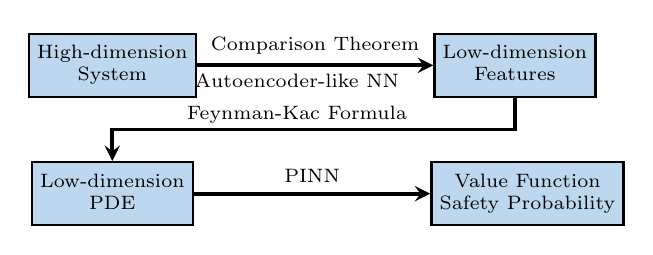
\begin{tikzpicture}[
    node distance = 4cm,
    node/.style={circle, fill=#1, inner sep=2pt, minimum size=0.7cm}, 
    edge/.style={-stealth, #1}
]

% 
\node[rectangle, draw=black, fill = newblue,line width = 0.3mm, minimum height=0.8cm,minimum width=2cm,inner sep=-3pt] (hds){\scriptsize \begin{tabular}{cc}
High-dimension \\ System
\end{tabular}};

\node[rectangle, draw=black, fill = newblue,line width = 0.3mm, minimum height=0.8cm,minimum width=2cm,inner sep=-3pt][right = 3cm of hds] (ldf){\scriptsize \begin{tabular}{cc}
Low-dimension \\ Features
\end{tabular}};


\node[rectangle, draw=black, fill = newblue,line width = 0.3mm, minimum height=0.8cm,minimum width=2cm,inner sep=-3pt][below = 0.8cm of hds] (pde){\scriptsize \begin{tabular}{cc}
Low-dimension \\ PDE
\end{tabular}};

\node[rectangle, draw=black, fill = newblue,line width = 0.3mm, minimum height=0.8cm,minimum width=2cm,inner sep=-3pt][right = 3cm of pde] (vfsp){\scriptsize \begin{tabular}{cc}
Value Function \\ Safety Probability
\end{tabular}};


%Edges
% \draw[edge=black,line width = 0.5mm] (hds) -> (pdf);

\draw [edge=black,line width = 0.5mm] (hds) -- (ldf) node[midway,above] {\scriptsize Comparison Theorem};

\node[rectangle][above left= -0.9cm and 0.1cm of ldf] (ct){\scriptsize \begin{tabular}{cc}
\color{black}{Autoencoder-like NN}
\end{tabular}};

% \draw [edge=black,line width = 0.3mm] (pdf) -- (pde) node[midway,above] {\scriptsize Comparison theorem};
\draw [edge=black,line width = 0.5mm, draw] (ldf.south) -- ++(0,-0.4) node(midway, north){} -| (pde.north);

\node[rectangle][below left= -0.05cm and 0cm of ldf] (ct){\scriptsize \begin{tabular}{cc}
\color{black}{Feynman-Kac Formula}
\end{tabular}};

% \node[rectangle][below left= 0.28cm and -0.5cm of pdf] (ct){\scriptsize \begin{tabular}{cc}
% \color{black}{Feynman-Kac Lemma}
% \end{tabular}};

\draw [edge=black,line width = 0.5mm] (pde) -- (vfsp) node[midway, above] {\scriptsize PINN};

\end{tikzpicture}
    \caption{The procedure diagram of the proposed method.}
    \label{fig:flowchart}
\end{figure}


\subsection{Comparison Theorem for Feature Identification}
We assume the low-dimensional feature can be represented by a smooth function $p: \mathbb{R}^n \rightarrow \mathbb{R}$. Here, we use comparison theorem~\cite[Theorem 3.1]{ikeda1977comparison} to find the stochastic process $\xi$ that describes the exact evolution of $p(x)$.
We introduce the operator $\mathcal{A}$ as
\begin{equation}
\label{eq:def_L}
\begin{aligned}
\mathcal{A}^U(\cdot)(x) & =\frac{\partial(\cdot)}{\partial x}(x) f(x)+ \frac{\partial (\cdot)}{\partial x}(x) \sigma(x) U + \\
& \qquad \frac{1}{2} \operatorname{Tr}\left(\frac{\partial^2(\cdot)}{\partial x^2}(x) \sigma(x) \sigma(x)^\top\right),
\end{aligned}
\end{equation}
where $U: \mathbb{R}^n \rightarrow \mathbb{R}^m$ is the control policy that maps the state to the control input, and we define
\begin{equation}
    a(x)=\sum_{i, j, k} \sigma_k^i(x) \sigma_k^j(x) \frac{\partial p}{\partial x_i}(x) \frac{\partial p}{\partial x_j}(x), \; b(x)=\frac{\mathcal{A}^U p(x)}{a(x)},
\end{equation}
where $\sigma_k^i(x)$ is the $(i,k)$-th element of the diffusion coefficient $\sigma(x)$.
For value function estimation, we consider $\mathcal{A}^0$ for the uncontrolled process where $U \equiv 0$, and for safety probability estimation, we consider $\mathcal{A}^{\mathcal{N}}$ where $U = \mathcal{N}$ is the nominal control policy.
Additionally, let $\xi \in I \subset \mathbb{R}$ be a scalar variable, where $I$ is the range of the feature $p(x)$. Using similar notation employed in~\cite{ikeda1977comparison}, consider
\begin{equation}
\label{eq:a_b_def}
\begin{aligned}
    a^{+}(\xi) = \sup _{x: p(x)=\xi} a(x), & \quad a^{-}(\xi) = \inf _{x: p(x)=\xi} a(x) \\
    b^{+}(\xi)= \sup _{x: p(x)=\xi} b(x), & \quad b^{-}(\xi)=\inf _{x: p(x)=\xi} b(x)
\end{aligned}
\end{equation}
\begin{assumption}
\label{asm:match_upper_lower_bound}
We assume that the feature function $p(x)$ satisfies that $a^{+}(\xi) = a^{-}(\xi) = \alpha(\xi)$ and $b^{+}(\xi) = b^{-}(\xi) = \beta(\xi)$, $\forall \xi \in I$.
\end{assumption}
\begin{assumption}
\label{asm:continuity-condition-on-a-and-b}
The functions $\alpha(\xi)$ and $\beta(\xi)$ are globally Lipschitz continuous in $\xi \in I \subset \mathbb{R}$.
Moreover, $a(x) > 0$, $\forall x \in \mathbb{R}^{n}$.
\end{assumption}

\begin{theorem}
\label{thm:comparison_lemma}
Given Assumptions~\ref{asm:match_upper_lower_bound} and~\ref{asm:continuity-condition-on-a-and-b} hold, $p(x_t)$ with $x_t$ being sampled from system~\eqref{eq:continuous_dynamics} is characterized by the following stochastic process
\begin{equation}
\label{eq:one_dim_xi_process}
    d \xi_t = \alpha\left(\xi_t\right) \beta\left(\xi_t\right) d t + \sqrt{\alpha\left(\xi_t\right)} d \tilde{B}_t,
\end{equation}
with $\xi_0 = p(x_0)$, and $\tilde{B}_t$ being a one-dimensional standard Wiener process.
\end{theorem}
\begin{proof}
    See appendix.
\end{proof}
Assumption~\ref{asm:match_upper_lower_bound} gives the conditions for the upper and lower bounds to match with the actual value $\alpha$ and $\beta$, thus a single stochastic process $\xi$ can be derived.
Till here, we have found the one-dimensional process~\eqref{eq:one_dim_xi_process} that characterizes the evolution of the feature of the high-dimensional system.

\subsection{PDE for Value Function with Feynman-Kac}
\label{sec:Feynman_Kac_PDE}
In this section, we describe how to estimate the value function with the solution of a low-dimensional PDE.
We consider $p(x) = c(x)$, \ie the feature of the high-dimensional system is the value of the running cost on state.
We set
\begin{equation}
\label{eq:V_exp_transformation}
    V(x, t)=-\log \varphi(x, t).
\end{equation}
Let $\xi = p(x)$, then from~\eqref{eq:value_function_free_energy} we have
\begin{equation}
\label{eq:xi_value_function}
\begin{aligned}
    \varphi(x, t) %& = \mathbb{E} \left[\exp \left(-\int_t^T c\left(x_\tau\right) d \tau - c(x_T)\right)  \mid x_t=x\right] \\
    & = \mathbb{E} \left[\exp \left(-\int_t^T \xi_\tau d \tau - \xi_T\right)  \mid \xi_t=\xi\right]
\end{aligned}
\end{equation}
With that, we apply Feynman-Kac formula~\cite{del2004feynman} on~\eqref{eq:xi_value_function} and~\eqref{eq:one_dim_xi_process} and get $\varphi(x, t)$ is the solution of the following two-dimensional PDE
\begin{equation}
\label{eq:one_dim_PDE}
\begin{aligned}
    W_{\varphi}(\xi,t) := & \frac{\partial \varphi}{\partial t}(\xi, t) + \alpha(\xi, t)\beta(\xi, t)\frac{\partial \varphi}{\partial \xi}(\xi, t) \\
    & +\frac{1}{2} \alpha(\xi, t) \frac{\partial^2 \varphi}{\partial \xi^2}(\xi, t) - \xi \varphi(\xi, t)=0,
\end{aligned}
\end{equation}
with initial (terminal) condition
\begin{equation}
\label{eq:one_dim_PDE_ic}
    \varphi(\xi, T) = \exp(-\frac{1}{2}\xi).
\end{equation}

\subsection{PDE for Safety Probability}
In this section, we describe how to estimate the safety probability with the solution of a low-dimensional PDE. We consider $p(x) = \phi(x)$, \ie the feature of the high-dimensional system is the value of the barrier function for the state. Then we have
\begin{equation}
\label{eq:safety_prob_hitting_time}
\begin{aligned}
    & \quad F(x,t) = \pr\left(x_\tau \in \safe, \forall \tau\in [0,t] \mid x_0 =x \right) \\
    & = \pr\left(\min_{0\leq \tau \leq t} \phi(x_\tau) \geq 0\right) = \pr\left(\min_{0\leq \tau \leq t} p(x_\tau) \geq 0\right) \\
    & = \pr\left(\min_{0\leq \tau \leq t} \xi_\tau \geq 0\right).
\end{aligned}
\end{equation}
The well-known results on the probability distribution of the first hitting time~\cite{patie2008first} allow us to obtain~\eqref{eq:safety_prob_hitting_time} as a solution to the two-dimensional PDE given by
\begin{equation}
\label{eq:one_dim_PDE_safe_prob}
\begin{aligned}
    W_{F}(\xi,t) := & \frac{\partial F}{\partial t}(\xi, t) - \alpha(\xi, t)\beta(\xi, t)\frac{\partial F}{\partial \xi}(\xi, t) \\
    & \quad - \frac{1}{2} \alpha(\xi, t) \frac{\partial^2 F}{\partial \xi^2}(\xi, t) =0,
\end{aligned}
\end{equation}
with boundary and initial conditions
\begin{equation}\label{eq:safe_PDE_ic_bc}
      F(\xi, 0)  = 1, \,\, \xi > 0; \quad F(0, t)  = 0, \,\, t > 0.
\end{equation}



\subsection{Physic-informed Learning}

In this section, we will introduce a physics-informed learning pipeline to solve the PDE for the value function~\eqref{eq:one_dim_PDE} and the PDE for safety probability~\eqref{eq:one_dim_PDE_safe_prob}. For conciseness, we will focus on the case of value function estimation, as adaptation to safety probability estimation is trivial where one just need to replace the variables and the governing PDE.

From~\eqref{eq:path_integral_MC_estimation}, we can estimate the value function using path integral control by sampling the uncontrolled process. However, the path integral MC is not sample efficient when we want to know the value function on the entire space, especially for a large horizon $T$. Further, efficiently solving the value function PDE~\eqref{eq:one_dim_PDE} using standard numerical methods is challenging.

To leverage the advantages of MC and PDE methods and to overcome their drawbacks, we propose a physics-informed neural network (PINN) to learn the mapping from the feature-time pair to the value function $\varphi$.
Fig.~\ref{fig:PINN diagram} shows the architecture of the PINN. The PINN takes the feature-time pair $(\xi,t)$ as the input, and outputs the value function prediction $\hat{\varphi}$, the feature and time derivatives $ \frac{\partial \hat \varphi}{\partial \xi}$ and $ \frac{\partial \hat \varphi}{\partial t}$, and the Hessian $ \frac{\partial^2 \hat \varphi}{\partial \xi^2}$, which come naturally from the automatic differentiation in deep learning frameworks such as PyTorch~\cite{paszke2019pytorch} and TensorFlow~\cite{abadi2016tensorflow}.
Assume the PINN is parameterized by $\boldsymbol\theta$, the loss function is defined as
\begin{equation}
\label{eq:PINN overall loss function}
    \mathcal{L}(\boldsymbol\theta) = \omega_p \mathcal{L}_p(\boldsymbol\theta) + \omega_d \mathcal{L}_d(\boldsymbol\theta),
\end{equation}
where
\begin{equation}
\label{eq:PINN loss functions}
\begin{aligned}
    \mathcal{L}_p(\boldsymbol\theta) & = \frac{1}{|\mathcal{P}|} \sum_{(\xi,t) \in \mathcal{P}} \|W_{\hat{\varphi}_{\boldsymbol\theta}}(\xi,t)\|_2^2, \\
    \mathcal{L}_d(\boldsymbol\theta) & = \frac{1}{|\mathcal{D}|} \sum_{(\xi,t) \in \mathcal{D}} \|\hat{\varphi}_{\boldsymbol\theta}(\xi,t) - \bar{\varphi}(\xi,t)\|_2^2.
\end{aligned}
\end{equation}
Here, $\bar{\varphi}$ is the training data, $\hat{\varphi}_{\boldsymbol\theta}$ is the prediction from the PINN, $\mathcal{P}$ and $\mathcal{D}$ are the training point sets for the physics model and external data, respectively. The loss function $\mathcal{L}$ consists of two parts, the physics model loss $\mathcal{L}_p$ and data loss $\mathcal{L}_d$. The physics model loss $\mathcal{L}_p$ measures the satisfaction of the PDE constraints for the learned output. It calculates the actual PDE equation value $W_{\hat{\varphi}_{\boldsymbol\theta}}$, which is supposed to be $0$, and use its 2-norm as the loss. The data loss $\mathcal{L}_d$ measures the accuracy of the prediction of PINN on the training data. It calculates the mean square error between the PINN prediction and the training data point as the loss. The overall loss function $\mathcal{L}$ is the weighted sum of the physics model loss and data loss with weighting coefficients $\omega_p$ and $\omega_d$.
Though out of the scope of this paper, theoretical analysis on the approximation error of PINNs and neural operators can be found in~\cite{wang2023generalizable, lu2021learning, kovachki2021universal}.

\begin{figure*}[t]
\begin{subfigure}[t]{0.65\textwidth}
\centering
\tikzstyle{line} = [draw, -latex']

\tikzset{
diagonal fill/.style 2 args={fill=#2, path picture={
\fill[#1, sharp corners] (path picture bounding box.south west) -|
                         (path picture bounding box.north east) -- cycle;}},
reversed diagonal fill/.style 2 args={fill=#2, path picture={
\fill[#1, sharp corners] (path picture bounding box.north west) |- 
                         (path picture bounding box.south east) -- cycle;}}
}

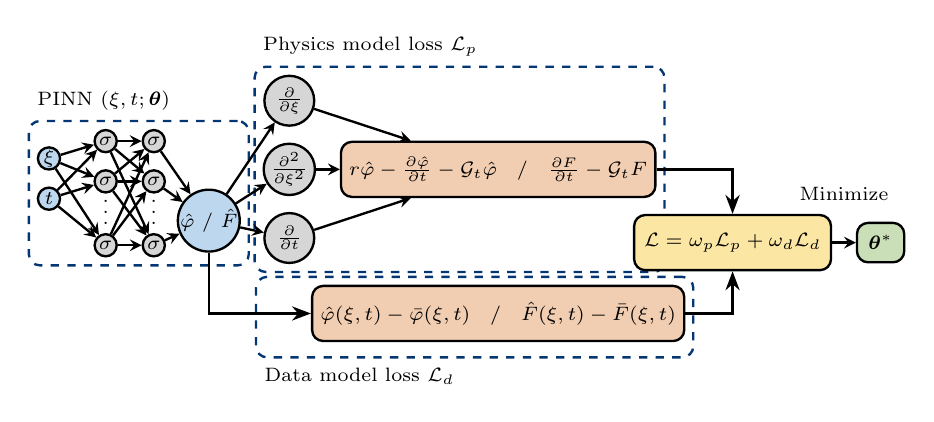
\begin{tikzpicture}[
    node distance = 1.2cm,
    fontscale/.style = {font=\scriptsize},
    node/.style={circle, fill=#1, inner sep=0pt, minimum size=0.1cm}, 
    edge/.style={-stealth, #1},
    arr/.style = {semithick, -Stealth}
]
    
    %Block 1
    %Nodes
    \node[circle, fill = newblue, draw=black, line width=0.3mm, inner sep=0pt, minimum size=8pt]  (xi) {\scriptsize $\xi$};
    \node[circle, fill = newblue, draw=black, line width=0.3mm, inner sep=0pt, minimum size=8pt] (t) [below = 0.2cm of xi] {\scriptsize $t$};

    \node[circle, fill = newgray, draw=black, line width=0.3mm, inner sep=0pt, minimum size=8pt]  (sigma1)[above right = -0cm and 0.5cm of xi] {\scriptsize $\sigma$};
    \node[circle, fill = newgray, draw=black, line width=0.3mm, inner sep=0pt, minimum size=8pt]  (sigma2)[below = 0.2cm of sigma1] {\scriptsize $\sigma$};
    \node[circle, fill = newgray, draw=black, line width=0.3mm, inner sep=0pt, minimum size=8pt]  (sigma3)[below = 0.5cm of sigma2] {\scriptsize $\sigma$};

    \node[circle, fill = newgray, draw=black, line width=0.3mm, inner sep=0pt, minimum size=8pt]  (sigma4)[right = 0.3cm of sigma1] {\scriptsize $\sigma$};
    \node[circle, fill = newgray, draw=black, line width=0.3mm, inner sep=0pt, minimum size=8pt]  (sigma5)[right = 0.3cm of sigma2] {\scriptsize $\sigma$};
    \node[circle, fill = newgray, draw=black, line width=0.3mm, inner sep=0pt, minimum size=8pt]  (sigma6)[right = 0.3cm of sigma3] {\scriptsize $\sigma$};

    \node[circle, fill = newblue, draw=black, line width=0.3mm, inner sep=0pt, minimum size=8pt]  (phi)[below right = 0.1cm and 0.3cm of sigma5] {\scriptsize $\hat \varphi$ / $\hat F$};


    %Edges
    % \draw[edge=blue,line width=0.5mm] (A) ->node[above]{$p$} (B);
    \draw[edge,line width=0.3mm] (xi) -> (sigma1);
    \draw[edge,line width=0.3mm] (xi) -> (sigma2);
    \draw[edge,line width=0.3mm] (xi) -> (sigma3);

    \draw[edge,line width=0.3mm] (t) -> (sigma1);
    \draw[edge,line width=0.3mm] (t) -> (sigma2);
    \draw[edge,line width=0.3mm] (t) -> (sigma3);

    \draw[edge,line width=0.3mm] (sigma1) -> (sigma4);
    \draw[edge,line width=0.3mm] (sigma1) -> (sigma5);
    \draw[edge,line width=0.3mm] (sigma1) -> (sigma6);

    \draw[edge,line width=0.3mm] (sigma2) -> (sigma4);
    \draw[edge,line width=0.3mm] (sigma2) -> (sigma5);
    \draw[edge,line width=0.3mm] (sigma2) -> (sigma6);

    \draw[edge,line width=0.3mm] (sigma3) -> (sigma4);
    \draw[edge,line width=0.3mm] (sigma3) -> (sigma5);
    \draw[edge,line width=0.3mm] (sigma3) -> (sigma6);

    \node at ($(sigma2)!.35!(sigma3)$) {\scriptsize \vdots};
    \node at ($(sigma5)!.35!(sigma6)$) {\scriptsize \vdots};

    \draw[edge,line width=0.3mm] (sigma4) -> (phi);
    \draw[edge,line width=0.3mm] (sigma5) -> (phi);
    \draw[edge,line width=0.3mm] (sigma6) -> (phi);

    \node[rectangle, draw=cmublue, fit=(xi) (sigma1) (sigma3) (phi), rounded corners, dashed, line width=0.3mm, inner sep=1mm] (block1) {};
    \node[above right] at (block1.north west){\scriptsize PINN $(\xi,t;\boldsymbol\theta)$};

    

    % block2
    \node[circle, fill = newgray, draw=black, line width=0.3mm, inner sep=0pt, minimum size=18pt]  (par1)[above right= 1cm and 0.5cm of phi] {\scriptsize $\frac{\partial}{\partial\xi}$};
    \node[circle, fill = newgray, draw=black, line width=0.3mm, inner sep=0pt, minimum size=18pt]  (par2)[below= 0.2cm of par1] {\scriptsize $\frac{\partial^2}{\partial\xi^2}$};
PF    \node[circle, fill = newgray, draw=black, line width=0.3mm, inner sep=0pt, minimum size=18pt]  (par3)[below= 0.2cm of par2] {\scriptsize $\frac{\partial}{\partial t}$};

    \node[rectangle, fill = neworange, draw=black, line width=0.3mm, inner sep=3pt, minimum height = 0.7cm, minimum width = 2.5cm, rounded corners]  (eq1)[right= 0.3cm of par2] {\scriptsize $r \hat \varphi -\frac{\partial \hat \varphi}{\partial t}-\mathcal{G}_t \hat \varphi$ \: / \: $\frac{\partial F}{\partial t}-\mathcal{G}_t F$};

    \draw[edge,line width=0.3mm] (par1) -> (eq1);
    \draw[edge,line width=0.3mm] (par2) -> (eq1);
    \draw[edge,line width=0.3mm] (par3) -> (eq1);

    \node[rectangle, draw=cmublue, fit=(par1) (par2) (par3) (eq1), rounded corners, dashed, line width=0.3mm, inner sep=1mm] (block2) {};
    \node[above right] at (block2.north west){\scriptsize Physics model loss $\mathcal{L}_p$};

    % block3
    \node[rectangle, fill = neworange, draw=black, line width=0.3mm, inner sep=3pt, minimum height = 0.7cm, minimum width = 2.5cm, rounded corners] (eq2)[below= 1.1cm of eq1] {\scriptsize $\hat{\varphi}(\xi,t) - \bar{\varphi}(\xi,t)$ \: / \: $\hat{F}(\xi,t) - \bar{F}(\xi,t)$};
    \node[circle, inner sep=0pt, minimum size=18pt] (par4)[below= 1.3cm of par2] {};
    \node[rectangle, draw=cmublue, fit=(par4) (eq2), rounded corners, dashed, line width=0.3mm, inner sep=1mm] (block3) {};
    \node[below right] at (block3.south west){\scriptsize Data model loss $\mathcal{L}_d$};

    
    \draw[edge,line width=0.3mm] (phi) -> (par1);
    \draw[edge,line width=0.3mm] (phi) -> (par2);
    \draw[edge,line width=0.3mm] (phi) -> (par3);
    % \draw[edge,line width=0.3mm] (phi) -> (eq2);
    \draw [arr,line width=0.3mm] (phi) |- (eq2);

    % loss
    \node[rectangle, fill = newyellow, draw=black, line width=0.3mm, inner sep=0pt, minimum height = 0.7cm, minimum width = 2.5cm, rounded corners]  (loss)[below right= 0.2cm and -0.3cm of eq1] {\scriptsize  $\mathcal{L} = \omega_p \mathcal{L}_p + \omega_d \mathcal{L}_d$};
    \draw [arr,line width=0.3mm] (eq1) -| (loss);
    \draw [arr,line width=0.3mm] (eq2) -| (loss);

    % theta
    \node[rectangle, fill = newgreen, draw=black, line width=0.3mm, inner sep=0pt, minimum height = 0.5cm, minimum width = 0.6cm, rounded corners]  (theta)[right= 0.3cm of loss] {\scriptsize $\boldsymbol\theta^*$};
    % \draw[edge,line width=0.3mm, label = minimize] (loss) -> (theta);
    \path[-stealth,draw,line width=0.3mm](loss) edge node[above=0.4cm] {\scriptsize Minimize} (theta);
    

\end{tikzpicture}

 
\phantomsubcaption
\label{fig:PINN diagram}
\end{subfigure}
\hfill
\begin{subfigure}[t]{0.35\textwidth}
\centering
\phantomsubcaption
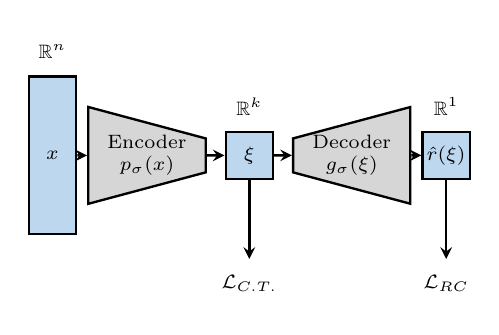
\begin{tikzpicture}[
    node distance = 4cm,
    node/.style={circle, fill=#1, inner sep=2pt, minimum size=0.7cm}, 
    edge/.style={-stealth, #1}
]

% x
\node[rectangle, draw, line width=0.3mm, fill = newblue, minimum height=2cm,minimum width=0.6cm,inner sep=0pt] at (0,0) (x){\scriptsize $x$};

\node[rectangle, minimum height=0.6cm,minimum width=0.6cm,inner sep=0pt] (r1)[above = 0cm of x]{\scriptsize $\mathbb{R}^n$};

% encoder
\node[trapezium,draw,line width=0.3mm,trapezium angle=75, minimum width = 1.23cm, fill = newgray, 
    minimum height = 1.3cm, rotate = -90, inner sep = -3pt](encoder)at (1.2,0) {\scriptsize \rotatebox{90}{\begin{tabular}{cc} Encoder \\ $p_\sigma (x)$ \end{tabular}}};

% xi
\node[rectangle, draw, line width=0.3mm, fill = newblue, minimum height=0.6cm,minimum width=0.6cm,inner sep=0pt] at (2.5,0) (xi){\scriptsize $\xi$};

\node[rectangle, minimum height=0.6cm,minimum width=0.6cm,inner sep=0pt] (r2)[above = 0cm of xi]{\scriptsize $\mathbb{R}^k$};

\node[rectangle, minimum height=0.6cm,minimum width=0.6cm,inner sep=0pt] (l1)[below = 1cm of xi]{\scriptsize $\mathcal{L}_{C.T.}$};

% decoder
\node[trapezium,draw,line width=0.3mm,trapezium angle=75, minimum width = 1.23cm, fill = newgray, 
    minimum height = 1.3cm, rotate = 90, inner sep = -3pt](decoder)at (3.8,0) {\scriptsize \rotatebox{-90}{\begin{tabular}{cc} Decoder \\ $g_\sigma (\xi)$ \end{tabular}}};

% g
\node[rectangle, draw, line width=0.3mm, fill = newblue, minimum height=0.6cm, minimum width=0.6cm,inner sep=0pt] at (5,0) (f){\scriptsize $\hat{r}(\xi)$};

\node[rectangle, minimum height=0.6cm,minimum width=0.6cm,inner sep=0pt] (r3)[above = 0cm of f]{\scriptsize $\mathbb{R}^1$};

\node[rectangle, minimum height=0.6cm,minimum width=0.6cm,inner sep=0pt] (l2)[below = 1cm of f]{\scriptsize $\mathcal{L}_{RC}$};

% arrows
\draw[edge,line width=0.3mm] (x) -> (encoder);
\draw[edge,line width=0.3mm] (encoder) -> (xi);
\draw[edge,line width=0.3mm] (xi) -> (decoder);
\draw[edge,line width=0.3mm] (decoder) -> (f);
\draw[edge,line width=0.3mm] (xi) -> (l1);
\draw[edge,line width=0.3mm] (f) -> (l2);
\end{tikzpicture}
\label{fig:AE diagram}
\end{subfigure}
\caption{(\subref{fig:PINN diagram}) The training scheme of the physics-informed neural network (PINN).
        (\subref{fig:AE diagram}) Autoencoder-like network architecture.}
\end{figure*}


\begin{remark}
For finding the optimal control, one can further enhance the sample complexity using path integral control together with value function prediction from the PINN. Denote $\hat{V}$ as the PINN value function prediction, we can initially estimate the optimal control from~\eqref{eq:optimal_control_from_V} with $\hat{u}(x,t) =  -\sigma\left(x\right)^\top \nabla \hat{V}\left(x, t\right)$. Then we can refine the optimal control using importance sampling~\cite{thijssen2015path} with the following procedure
\begin{equation}
\label{eq:optimal_control_IS}
\begin{aligned}
& u^{\star}(x, t)-\hat{u}(x, t)= \\
& \lim _{s \searrow t} \frac{\mathbb{E}^{P}\left\{\exp \left\{-S^{\hat{u}}(t)\right\} \int_t^s d W_\tau \mid x_t=x\right\}}{(s-t) \mathbb{E}^{P}\left\{\exp \left\{-S^{\hat{u}}(t)\right\} \mid x_t=x\right\}}
\end{aligned}
\end{equation}
where $P$ is the process with regard to $\hat{u}$ and
\begin{equation}
\label{eq:cost_function_u_hat}
    S^{\hat{u}}(t)=\int_t^T w\left(x_\tau, \hat{u}_\tau\right)
    d \tau+\int_t^T \hat{u}_\tau^{\top} d W_\tau+c\left(x_T\right).
\end{equation}
Essentially, one can use the sampled cost function~\eqref{eq:cost_function_u_hat} with control policy $\hat{u}$ to estimate the optimal control policy $u^\star$ with~\eqref{eq:optimal_control_IS}. The sample complexity for estimating the expectation in~\eqref{eq:optimal_control_IS} is much lower than the naive estimation with~\eqref{eq:path_integral_MC_estimation} and~\eqref{eq:optimal_control_from_V} due to the fact that path generated from $\hat{u}$ is much closer to the optimal path. The importance sampling theory provides theoretical analysis on the improvement of the sample complexity~\cite{thijssen2015path}.

\end{remark}


\subsection{Generalization: Arbitrary Feature Dimension}
In this section we generalize the previous results such that the representation of the system can be of arbitrary dimension. The procedure consists of two key steps. First, we use comparison theorem to find a multidimensional representation of the value function and the associated multidimensional process, \ie $\xi = [\xi^{(1)}, \xi^{(2)}, \cdots, \xi^{(k)}]^\top$ where $k$ is the dimension of the reduced representation. Then, we apply the high-dimensional Feynman-Kac formula~\cite[Theorem 1.3.17]{pham2009continuous} to
transform the stochastic process $\xi$ to a $k$-dimensional PDE which can be solved by the PINN.

For the first step, we find functions $p(x) = [p_1(x), p_2(x), \cdots, p_k(x)]^\top$ as the low dimensional representation of the original system.
We define $a_i^{+-}$ and $b_i^{+-}$ similar to~\eqref{eq:a_b_def} and assume Assumption~\ref{asm:match_upper_lower_bound} and~\ref{asm:continuity-condition-on-a-and-b} hold for $\forall i$.
Then from the comparison theorem, we can find stochastic processes
\begin{equation}
\label{eq:xi_process_high_dim}
    d \xi^{(i)}_t=\alpha_i\left(\xi^{(i)}_t\right) \beta_i\left(\xi^{(i)}_t\right) d t+\sqrt{\alpha_i\left(\xi^{(i)}_t\right)} d \tilde{B}^{(i)}_t
\end{equation}
for $i = 1,2,\cdots, k$ that characterize $p_i(x)$, where $\tilde{B}^{(i)}_t$ is one-dimensional standard Wiener processes.

\begin{assumption}
\label{asm:value_function_representation}
    For value function estimation, we assume the running-cost can be represented by the following function
\begin{equation}
\label{eq:cost_function_xi}
    c(x) = r(\xi) = r\left(p_1(x), p_2(x), \cdots, p_k(x)\right)
\end{equation}
where $r:\mathbb{R}^{k} \rightarrow \mathbb{R}$ is a continuous function.
\end{assumption}
Then
\begin{equation}
\label{eq:xi_value_function_high_dim}
\begin{aligned}
    \varphi(x, t) %& = \mathbb{E} \left[\exp \left(-\int_t^T c\left(x_\tau\right) d \tau - c(x_T)\right)  \mid x_t=x\right] \\
    & = \mathbb{E} \left[\exp \left(-\int_t^T r(\xi_\tau) d \tau - r(\xi_T)\right)  \mid \xi_t=\xi\right].
\end{aligned}
\end{equation}
From the high-dimensional Feynman-Kac formula~\cite[Theorem 1.3.17]{pham2009continuous}, we have $\varphi$ as the solution of the following PDE
\begin{equation}
\begin{aligned}
r \varphi -\frac{\partial \varphi}{\partial t}-\mathcal{G}_t \varphi =0&, & & \text { on } \mathbb{R}^k \times [0, T) \\
\varphi(\cdot,T) =\exp(-r(\cdot))&, & & \text { on } \mathbb{R}^k,
\end{aligned}
\end{equation}
where $r$ is given by~\eqref{eq:cost_function_xi} and
\begin{equation}
\label{eq:Gt_def}
   \mathcal{G}_t  (\cdot)=\alpha\left(\xi_t\right) \beta\left(\xi_t\right) \cdot \frac{\partial (\cdot)}{\partial \xi}
    +\frac{1}{2} \operatorname{Tr}\left(\mathbf{a}\left(\xi_t\right) \frac{\partial^2 (\cdot)}{\partial \xi^2}
    \right),
\end{equation}
with
\begin{equation}
    \alpha\left(\xi_t\right) \beta\left(\xi_t\right) = \begin{bmatrix}
    \alpha_1\left(\xi^{(1)}_t\right) \beta_1\left(\xi^{(1)}_t\right) \\
    \alpha_2\left(\xi^{(2)}_t\right) \beta_2\left(\xi^{(2)}_t\right) \\
    \vdots \\
    \alpha_k\left(\xi^{(k)}_t\right) \beta_k\left(\xi^{(k)}_t\right)
    \end{bmatrix},
\end{equation}
and
\begin{equation}
    \mathbf{a}\left(\xi_t\right) = \begin{bmatrix}
    \alpha_1\left(\xi_t\right) &  &  \\
    & \alpha_2\left(\xi_t\right) &  &  \\
    &  & \ddots &  \\
    &  &  & \alpha_k\left(\xi_t\right) \\
    \end{bmatrix}.
\end{equation}


\begin{assumption}
\label{asm:barrier_function_representation}
Similarly, for safety probability estimation, we assume the barrier function can be represented by the following function
\begin{equation}
\label{eq:barrier_function_xi}
    \phi(x) = r(\xi) = r\left(p_1(x), p_2(x), \cdots, p_k(x)\right),
\end{equation}
where $r:\mathbb{R}^{k} \rightarrow \mathbb{R}$ is a continuous function.
\end{assumption}
Then the safety probability can be written as
\begin{equation}
\label{eq:xi_barrier_function_high_dim}
\begin{aligned}
    F(x,t) = \pr\left(\min_{0\leq \tau \leq t} \phi(x_\tau) \geq 0\right)  = \pr\left(\min_{0\leq \tau \leq t} r(\xi_\tau) \geq 0\right).
\end{aligned}
\end{equation}
We define $\mathcal{B} = \left\{\xi: r(\xi) \geq 0\right\}$. From the probability distribution of hitting time~\cite{patie2008first} we have that~\eqref{eq:xi_barrier_function_high_dim} can be characterized by the solution of the following PDE
\begin{equation}
    \frac{\partial F}{\partial t}-\mathcal{G}_t F =0,  \text {on }[0, T) \times \mathbb{R}^n
\end{equation}
\begin{equation}
   F(\xi,0)  =1, \,\, \xi\in\mathcal{B}; \quad F(\xi,t)  =0, \,\, \xi \in \partial \mathcal{B}.
\end{equation}





\begin{remark}
\label{rmk:low_dim_representation}
    The Assumptions~\ref{asm:value_function_representation} or~\ref{asm:barrier_function_representation} where the running-cost can be represented by~\eqref{eq:cost_function_xi} or the barrier function can be represented by~\eqref{eq:barrier_function_xi} is a necessary condition for the proposed method to work. The high-dimensional system must admit a low-dimensional representation of its value function/safety probability.
\end{remark}


\subsection{Deep Learning for Feature Identification}
For high dimensional systems with complex structure, deriving features $p_1, p_2, \ldots, p_k$ such that Assumptions 2 and 3 hold is a challenging problem.  Thus, we propose an autoencoder-like neural network (Fig. \ref{fig:AE diagram}) to automatically identify lower-dimensional features that meet the bounding  requirements of Assumption~\ref{asm:match_upper_lower_bound} and sufficiently represent the cost/barrier function (Remark~\ref{rmk:low_dim_representation}). The network takes an input state $x\in\mathbb{R}^n$ and outputs 1) a low-dimensional representation $\xi\in\mathbb{R}^k$ via the encoder $p_\sigma(x)$, and 2) the function $\hat{r}(\xi)\in\mathbb{R}$ via the decoder $g_\sigma(\xi)$. We use $\boldsymbol \theta$ as the parameters of the autoencoder-like model. The loss function is defined as
\begin{equation}\label{eq: AE Loss}
    \mathcal{L}_{AE}(\boldsymbol\theta) = w_{RC}\mathcal{L}_{RC}(\boldsymbol\theta) + w_{C.T.}\mathcal{L}_{C.T.}(\boldsymbol\theta)
\end{equation}
where
\begin{align}
    \mathcal{L}_{RC}(\boldsymbol\theta) &= \frac{1}{|\mathcal{X}|}\sum_{x\in\mathcal{X}}\left(c(x)-\hat{r}(\xi; \boldsymbol\theta)\right)^2, \label{eq: RC loss} \\
    \mathcal{L}_{C.T.}(\boldsymbol\theta) &= \frac{1}{k}\sum_{i=1}^k\frac{1}{|\mathcal{R}_i|}\sum_{\xi\in\mathcal{R}_i}\frac{1}{|\mathcal{M}_{\xi, i}|}\sum_{x\in\mathcal{M}_{\xi, i}} \label{eq: CT loss} \\
    & \quad \ldots ||\nabla a_i(x; \boldsymbol\theta) ||_2^2 + || \nabla b_i(x; \boldsymbol\theta)||_2^2 \nonumber
\end{align}
Here, $\mathcal{X}$ is the discretized state-space, $k$ is the dimension of the feature space, $\mathcal{R}_i$ is the range of $p_i$ and $\mathcal{M}_{\xi, i}=\{x: p_i(x; \boldsymbol\theta)=\xi\}$ is the set of $x$ that maps to the same value of $\xi\in\mathcal{R}_i$. The reconstruction loss $\mathcal{L}_{RC}$ measures how well the reconstruction $\hat{r}(\xi)$ represents $c(x)$ or $\phi(x)$, corresponding to Remark~\ref{rmk:low_dim_representation}. The comparison theorem loss $\mathcal{L}_{C.T.}$ enforces the condition that $a_i(x)$ and $b_i(x)$ are constant for all $x\in \mathcal{M}_{\xi, i}$, for each $\xi\in\mathcal{R}_i$, and for each feature $p_1,\ldots,p_k$. This is a sufficient condition to achieve Assumption~\ref{asm:match_upper_lower_bound}. The overall loss function is the weighted sum of the reconstruction loss and comparison theorem loss, where weights are chosen according to the desired strength and balance on the cost/barrier function reconstruction and the satisfaction of the comparison theorem. We refer readers to the appendix for more details about the algorithm.


\section{Experiments}
\label{sec:experiments}

In this section, we show experiment results of the proposed method with both qualitative and quantitative analysis.


\subsection{Value Function Estimation}

We consider a 1000-dimensional system for which we want a 2-dimensional representation of the optimal value function. The system dynamics is given by
\begin{equation}
\label{eq:1000d_system_experiment}
\begin{aligned}
    dx = & \bar A x dt+ \sigma ( udt + dw), \\
\end{aligned}
\end{equation}
where $x \in \mathbb{R}^{1000}$ is the state, $u \in \mathbb{R}^{1000}$ in the control, and $dw$ is the 1000-dimensional standard Wiener process. We set $\sigma = I_{1000}$ to be the identity matrix, and set $\bar A = \left[\begin{array}{l|l}
A & 0 \\
\hline 0 & A
\end{array}\right]$ where $A \in \mathbb{R}^{500 \times 500}$. Let $a_{i,j}$ be the entry of $A$ at $i$-th row and $j$-th column. We choose $A$ such that $a_{i,i} = 1.1$, $a_{i,(i+2) | 500} = a_{i,(i+4) | 500} = 0.1$ and $a_{i,(i+6) | 500} = a_{i,(i+8) | 500} = -0.1$ for $\forall i = 1,2, \cdots, 500$, where $|$ is the mod operator. The running cost function is assumed to be
\begin{equation}
\label{eq:1000d_system_experiment_cost}
    c(x) =
    \frac{1}{500}(\sum_{i=1}^{500} x_i)^2 + \frac{1}{500}(\sum_{j=501}^{1000}{x_j})^2.
\end{equation}
We pick two features of the state,
\begin{equation}
\label{eq:1000d_features}
    \xi_1 = p_1(x) = \sum_{i=1}^{500} x_i, \quad \xi_2 = p_2(x) = \sum_{j=501}^{1000} x_j.
\end{equation}
Then from~\eqref{eq:a_b_def}, we have
\begin{equation}
\label{eq:1000d_alpha_beta}
\begin{aligned}
    \alpha_1(\xi_1) = \alpha_2(\xi_2) = 500; \, \beta_1(\xi_1) = \frac{\xi_1}{500}, \ \beta_2(\xi_2) = \frac{\xi_2}{500},
\end{aligned}
\end{equation}
thus satisfying Assumptions~\ref{asm:match_upper_lower_bound} and~\ref{asm:continuity-condition-on-a-and-b}, and the running cost function can be written as
\begin{equation} \label{eq: r_xi_1000d}
    r(\xi) = \frac{1}{500}\xi_1^2 + \frac{1}{500}\xi_2^2.
\end{equation}
By the Feynman-Kac formula, we know that the exponential of the optimal value function $\varphi$ is the solution of the following PDE
\begin{align}
    & 0 = r(\xi)\mu
    - \frac{\partial \mu}{\partial t} -
    \alpha(\xi) \beta(\xi) \frac{\partial \mu}{\partial \xi} - \frac{1}{2} \operatorname{Tr} \left(
    \mathbf{a}(\xi) \frac{\partial^2 \mu}{\partial \xi^2} \right) \\
    & = \frac{\xi_1^2 + \xi_2^2}{500}\mu - \frac{\partial \mu}{\partial t} - \xi_1 \frac{\partial \mu}{\partial \xi_1} - \xi_2 \frac{\partial \mu}{\partial \xi_2} - \frac{\partial^2 \mu}{\partial \xi_1^2} - 250 \frac{\partial^2 \mu}{\partial \xi_2^2} \nonumber
\end{align}

\begin{equation}
    \mu(\xi, T) = \exp(- \frac{1}{500}\xi_1^2 - \frac{1}{500}\xi_2^2).
\end{equation}
With that, we generate data for $\bar \varphi(x,t)$ on spatial-temporal space $\Omega \times \mathbb{T} = [1,2]^2 \times [0,1.5]$, with grid size $d\xi = 0.1$ and $dt = 0.1$ and train the PINN on $\Omega \times \mathbb{T} = [1,2]^2 \times [1,1.5]$.
We use a PINN with 3 hidden layers and 32 neurons per layer to learn the value function $\hat \varphi$. The activation function is chosen as hyperbolic tangent function ($\tanh$). We use the Adam optimizer~\cite{kingma2014adam} for training with initial learning rate set as $0.001$. The PINN parameters $\boldsymbol\theta$ is initialized via Glorot uniform initialization and the weights in the loss function~\eqref{eq:PINN overall loss function} are set to be $\omega_p = \omega_d = 1$. The simulation is constructed based on the DeepXDE framework~\cite{lu2021deepxde}. Fig.~\ref{fig:value_func_visual_1000d} shows the estimated value function from the path integral MC and the proposed method. It can be seen that the proposed framework is able to estimate value functions accurately, while the path integral method has significantly more noise. Also, the computation time for training the PINN is significantly less than sampling path integral MC (80s v.s $\sim$3000s). Note that the PINN is able to estimate the value function at unseen regions in the state space and generalize to longer time horizons, as the testing data at $t = 0.5$ is not seen by the PINN during training.
We refer readers to the appendix for the safety probability estimation setting where similar results can be obtained.




\begin{figure}[t]
  \begin{subfigure}{0.49\columnwidth}
  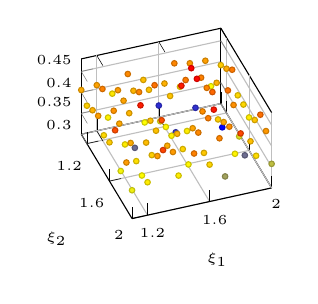
\begin{tikzpicture}
 
\begin{axis}[
% hide x axis,
% hide y axis,
% tick align=outside,
view/h=70,
view/v=50,
tick pos=left,
% x grid style={darkgray176},
% xlabel style={rotate=-10},
xlabel={\(\displaystyle \xi_2\)},
xtick = {1.2,1.6,2},
% xmin=1.0395, xmax=1.1605,
xtick style={color=black},
% y grid style={darkgray176},
% ylabel style={rotate=45},
ylabel={\(\displaystyle \xi_1\)},
ytick = {1.2,1.6,2},
% ymin=1.0395, ymax=1.1605,
ytick style={color=black},
% yticklabel style={anchor=center}
ztick = {0.3, 0.35, 0.4, 0.45},
zmin = 0.3, zmax = 0.48,
width=4cm,height=4cm,
font = \tiny, 
grid
]
 
\addplot3[
  mark=*,
  mark size=1pt,
  only marks,
  scatter,
  scatter/@post marker code/.code={%
  \endscope
},
%   scatter/@pre marker code/.code={%
%   \expanded{%
%   \noexpand\definecolor{thispointdrawcolor}{RGB}{\drawcolor}%
%   \noexpand\definecolor{thispointfillcolor}{RGB}{\fillcolor}%
%   }%
%   \scope[draw=thispointdrawcolor, fill=thispointfillcolor]%
% },
%   visualization depends on={value \thisrow{draw} \as \drawcolor},
%   visualization depends on={value \thisrow{fill} \as \fillcolor}
] table 
{
% x y   z
% 1.1 1.1   0.39946797
% 1.1 1.2 0.40073798
% }
x    y         z
1.1	1.1	0.40565765
1.1	1.2	0.40906673
1.1	1.3	0.38070724
1.1	1.4	0.41947888
1.1	1.5	0.39722215
1.1	1.6	0.327815  
1.1	1.7	0.42057389
1.1	1.8	0.4125304 
1.1	1.9	0.41043739
1.1	2.0	0.39177632
1.2	1.1	0.39057698
1.2	1.2	0.42240288
1.2	1.3	0.41134408
1.2	1.4	0.40181783
1.2	1.5	0.39592508
1.2	1.6	0.4028499 
1.2	1.7	0.38691981
1.2	1.8	0.32852271
1.2	1.9	0.37189909
1.2	2.0	0.40569639
1.3	1.1	0.4021314 
1.3	1.2	0.37647653
1.3	1.3	0.40863601
1.3	1.4	0.42108011
1.3	1.5	0.42933735
1.3	1.6	0.39541396
1.3	1.7	0.42539899
1.3	1.8	0.42294425
1.3	1.9	0.40247396
1.3	2.0	0.42562671
1.4	1.1	0.41106665
1.4	1.2	0.41515223
1.4	1.3	0.40118414
1.4	1.4	0.37091946
1.4	1.5	0.36558178
1.4	1.6	0.33109136
1.4	1.7	0.47613098
1.4	1.8	0.42098295
1.4	1.9	0.31857162
1.4	2.0	0.38683164
1.5	1.1	0.38704072
1.5	1.2	0.40674994
1.5	1.3	0.34074324
1.5	1.4	0.39740023
1.5	1.5	0.37438479
1.5	1.6	0.46459003
1.5	1.7	0.47303517
1.5	1.8	0.43332828
1.5	1.9	0.42910044
1.5	2.0	0.38717436
1.6	1.1	0.39256698
1.6	1.2	0.37941244
1.6	1.3	0.46470152
1.6	1.4	0.39593074
1.6	1.5	0.37578946
1.6	1.6	0.37891176
1.6	1.7	0.4175584 
1.6	1.8	0.3902694 
1.6	1.9	0.41664273
1.6	2.0	0.37877905
1.7	1.1	0.44378004
1.7	1.2	0.40528874
1.7	1.3	0.3980817 
1.7	1.4	0.44333453
1.7	1.5	0.40275016
1.7	1.6	0.40793259
1.7	1.7	0.42380686
1.7	1.8	0.4063768 
1.7	1.9	0.36389793
1.7	2.0	0.39502977
1.8	1.1	0.36884713
1.8	1.2	0.38433559
1.8	1.3	0.39053864
1.8	1.4	0.40482896
1.8	1.5	0.38869122
1.8	1.6	0.41995875
1.8	1.7	0.4666564 
1.8	1.8	0.41770006
1.8	1.9	0.34124801
1.8	2.0	0.43008697
1.9	1.1	0.41154597
1.9	1.2	0.37233469
1.9	1.3	0.41076619
1.9	1.4	0.41227455
1.9	1.5	0.37438566
1.9	1.6	0.3938453 
1.9	1.7	0.42059355
1.9	1.8	0.37538536
1.9	1.9	0.39709385
1.9	2.0	0.41333092
2.0	1.1	0.36769539
2.0	1.2	0.37862954
2.0	1.3	0.44736103
2.0	1.4	0.37825467
2.0	1.5	0.4228928 
2.0	1.6	0.38815098
2.0	1.7	0.35185788
2.0	1.8	0.44647427
2.0	1.9	0.38486582
2.0	2.0	0.3575396 
};
\end{axis}
 
\end{tikzpicture}


  \phantomsubcaption
  \end{subfigure}
  \begin{subfigure}{0.49\columnwidth}
  % \def\axisdefaultticklabel{$\pgfmathprintnumber{\tick}$}

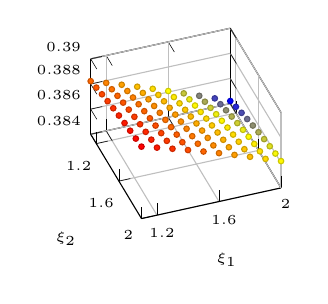
\begin{tikzpicture}
 
\begin{axis}[
% hide x axis,
% hide y axis,
% tick align=outside,
view/h=70,
view/v=50,
tick pos=left,
% x grid style={darkgray176},
% xlabel style={rotate=-10},
xlabel={\(\displaystyle \xi_2\)},
xtick = {1.2,1.6,2},
% xmin=1.0395, xmax=1.1605,
xtick style={color=black},
% y grid style={darkgray176},
% ylabel style={rotate=45},
ylabel={\(\displaystyle \xi_1\)},
ytick = {1.2,1.6,2},
% ymin=1.0395, ymax=1.1605,
ytick style={color=black},
% yticklabel style={anchor=center}
% zticklabels = {0.387,0.389,0.39, 0.392},
z tick label style={/pgf/number format/precision=3},
zmin=0.384, zmax=0.39,
ztick style={color=black},
width=4cm,height=4cm,
font = \tiny, 
grid
]
 
\addplot3[
  mark=*,
  mark size=1pt,
  only marks,
  scatter,
  scatter/@post marker code/.code={%
  \endscope
},
%   scatter/@pre marker code/.code={%
%   \expanded{%
%   \noexpand\definecolor{thispointdrawcolor}{RGB}{\drawcolor}%
%   \noexpand\definecolor{thispointfillcolor}{RGB}{\fillcolor}%
%   }%
%   \scope[draw=thispointdrawcolor, fill=thispointfillcolor]%
% },
%   visualization depends on={value \thisrow{draw} \as \drawcolor},
%   visualization depends on={value \thisrow{fill} \as \fillcolor}
] table 
{
% x y   z
% 1.1 1.1   0.39946797
% 1.1 1.2 0.40073798
% }
x    y         z
1.1	1.1	0.38822708
1.1	1.2	0.3878177 
1.1	1.3	0.3873986 
1.1	1.4	0.38696966
1.1	1.5	0.38653117
1.1	1.6	0.38608363
1.1	1.7	0.38562652
1.1	1.8	0.38516018
1.1	1.9	0.38468498
1.1	2.0	0.384201  
1.2	1.1	0.38845968
1.2	1.2	0.38805744
1.2	1.3	0.38764504
1.2	1.4	0.3872227 
1.2	1.5	0.38679066
1.2	1.6	0.38634878
1.2	1.7	0.38589743
1.2	1.8	0.3854364 
1.2	1.9	0.3849663 
1.2	2.0	0.38448724
1.3	1.1	0.3886749 
1.3	1.2	0.38827953
1.3	1.3	0.3878741 
1.3	1.4	0.3874583 
1.3	1.5	0.38703215
1.3	1.6	0.38659596
1.3	1.7	0.38615018
1.3	1.8	0.38569444
1.3	1.9	0.38522935
1.3	2.0	0.3847548 
1.4	1.1	0.3888729 
1.4	1.2	0.3884847 
1.4	1.3	0.38808578
1.4	1.4	0.38767618
1.4	1.5	0.38725623
1.4	1.6	0.3868259 
1.4	1.7	0.38638523
1.4	1.8	0.3859346 
1.4	1.9	0.38547435
1.4	2.0	0.38500416
1.5	1.1	0.38905445
1.5	1.2	0.38867337
1.5	1.3	0.3882807 
1.5	1.4	0.38787726
1.5	1.5	0.3874631 
1.5	1.6	0.3870382 
1.5	1.7	0.38660288
1.5	1.8	0.3861572 
1.5	1.9	0.38570136
1.5	2.0	0.3852356 
1.6	1.1	0.3892199 
1.6	1.2	0.38884515
1.6	1.3	0.3884591 
1.6	1.4	0.38806176
1.6	1.5	0.38765323
1.6	1.6	0.38723376
1.6	1.7	0.38680342
1.6	1.8	0.38636228
1.6	1.9	0.38591096
1.6	2.0	0.3854493 
1.7	1.1	0.38936958
1.7	1.2	0.38900158
1.7	1.3	0.38862154
1.7	1.4	0.38823003
1.7	1.5	0.387827  
1.7	1.6	0.38741255
1.7	1.7	0.38698718
1.7	1.8	0.3865506 
1.7	1.9	0.38610354
1.7	2.0	0.38564584
1.8	1.1	0.38950405
1.8	1.2	0.3891423 
1.8	1.3	0.38876835
1.8	1.4	0.3883825 
1.8	1.5	0.3879847 
1.8	1.6	0.38757548
1.8	1.7	0.3871547 
1.8	1.8	0.38672248
1.8	1.9	0.38627943
1.8	2.0	0.3858254 
1.9	1.1	0.38962328
1.9	1.2	0.38926792
1.9	1.3	0.3888999 
1.9	1.4	0.38851953
1.9	1.5	0.38812703
1.9	1.6	0.38772246
1.9	1.7	0.38730612
1.9	1.8	0.38687834
1.9	1.9	0.38643894
1.9	2.0	0.3859885 
2.0	1.1	0.38972837
2.0	1.2	0.38937902
2.0	1.3	0.38901663
2.0	1.4	0.3886415 
2.0	1.5	0.38825408
2.0	1.6	0.38785404
2.0	1.7	0.38744193
2.0	1.8	0.38701817
2.0	1.9	0.3865824 
2.0	2.0	0.38613522
};
\end{axis}
 
\end{tikzpicture}


  \phantomsubcaption
  \end{subfigure}
  \caption{Estimation of the exponential of value function at $t=0.5$ for a 1000-dimensional system by path integral MC (left), and by the proposed method (right).}
  \label{fig:value_func_visual_1000d}
\end{figure}






\subsection{Sample Complexity}
We further examine the computation complexity of the proposed method to show its advantages in sample efficiency. We consider the problem of value function estimation of a 3-dimensional system with similar dynamics and cost defined in~\eqref{eq:1000d_system_experiment} and~\eqref{eq:1000d_system_experiment_cost}.
Please see appendix for details of the settings.
Fig.~\ref{fig:sample_complexity} shows the percentage error of the estimated value function with different number of samples for path integral MC and PINN with and without using comparison theorem for dimension reduction. The path integral MC with dimension reduction has sample complexities that are one order less than MC without dimension reduction, which indicates the efficacy of the dimension reduction scheme from the comparison theorem. The PINN further reduces sample complexity and achieves the best trade-off between accuracy and computation.

\begin{figure}
    \centering
    % \pgfplotsset{width=7cm,height=3cm,compat=1.10}
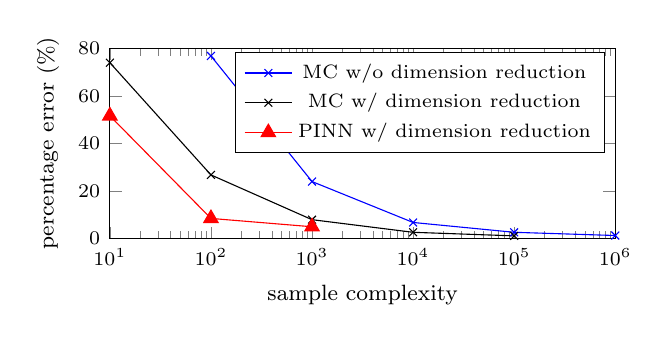
\begin{tikzpicture}
\begin{axis}[
    % x=0.5cm,
    % y=0.5cm/10,
    xlabel=\footnotesize{sample complexity},
    ylabel=\footnotesize{percentage error (\%)},
    xmode = log,
    xmin=10, xmax=10^6,
    ymin=0, ymax=80,
    % xtick={10^2,10^4,10^6},
    ytick={0,20,40,60,80},
    width=8cm,height=4cm,
    font = \scriptsize, 
            ]
\addplot[mark=x,blue] plot coordinates {
    (10^2,100*0.7675)
    (10^3,100*0.2399)
    (10^4,100*0.0680)
    (10^5,100*0.0267)
    (10^6,100*0.0132)    
};
\addlegendentry{MC w/o dimension reduction}

\addplot[color=black,mark=x,black]
    plot coordinates {
        (10^1,100*0.7392)
        (10^2,100*0.2678)
        (10^3,100*0.0797)
        (10^4,100*0.0267)
        (10^5,100*0.0117)
    };
\addlegendentry{MC w/ dimension reduction}

\addplot[color=red,mark=triangle*, mark size=3pt]
    plot coordinates {
        (10, 51.6)
        (100, 8.5)
        (1000,5)
    };
\addlegendentry{PINN w/ dimension reduction}
\end{axis}
\end{tikzpicture}
    \caption{Percentage error of the estimated value function with path integral MC.}
    \resolved{refine the plot, use pdf format}
    \label{fig:sample_complexity}
\end{figure}


\subsection{Feature Learning}
We verify our autoencoder-like network by learning the features and cost function in equations \eqref{eq:1000d_features} and~\eqref{eq: r_xi_1000d} for the 3-dimensional system described above. The network consists of 5 fully connected hidden layers of sizes 100, 10, 2, 10, 100, respectively, with the activation function as hyperbolic tangent. We use the Adam optimizer with initial learning rate set as 0.001. The parameters of the network are initialized via the Glorot uniform initialization. The weights in the loss function \eqref{eq: AE Loss} are set as $w_{RC}=1, \,w_{C.T.}=10$. The network is trained on a $[0, 1]^3$ state-space with grid size 0.01. The network successfully identified the features derived analytically in~\eqref{eq:3d_features} with $\mathrm{MSE}(\xi_1, \hat{\xi}_1)=0.2$ and $\mathrm{MSE}(\xi_2, \hat{\xi}_2)=0.06$.



\section{Conclusion}
\label{sec:conclusion}

We propose a unified framework for value function and safety probability estimation of high-dimensional stochastic systems. The novel dimensionality reduction technique uses the comparison theorem to generate low-dimensional stochastic processes that provide an exact characterization of the cost/barrier function, significantly improving sample complexity. We then transform the low-dimensional process into a low-dimensional PDE, and leverage physics-informed learning to generalize solutions into longer time horizons and unseen regions of state-space. We also achieve automatic feature identification through a specially designed autoencoder-like neural network. Experiment results show the efficacy of the proposed method. Future work includes application to multi-agent robotic control systems.




Hic qui voluptatum aspernatur autem pariatur adipisci reiciendis commodi mollitia, illum cum quae possimus ducimus, doloribus voluptates sed perferendis dolor aperiam dolore dignissimos ea pariatur ratione.Amet quas nihil optio accusantium maiores quos tempora sunt quod, soluta nulla natus harum nemo, et quas esse vitae accusantium fuga vero beatae, a beatae ut magni quam quasi?Temporibus cupiditate ullam sit dicta quo laudantium consequatur rerum illo, est similique reiciendis praesentium laboriosam in ipsum, eos asperiores minus doloremque natus.Eaque officiis in, dolor facere esse deleniti consequuntur praesentium hic assumenda officiis totam.Vel eos neque corporis accusantium id, rem commodi voluptates, perspiciatis possimus voluptate alias impedit quae?Error numquam minima inventore maiores sed, numquam earum dolorum, fugiat aliquam eaque tempore nisi ducimus, at a placeat pariatur non nulla ex eos harum odit similique amet, sapiente animi earum aliquam ratione repudiandae quod
\bibliography{main}

\end{document}